\documentclass[a4paper]{book}
\usepackage{makeidx}
\usepackage{graphicx}
\usepackage{multicol}
\usepackage{float}
\usepackage{listings}
\usepackage{color}
\usepackage{ifthen}
\usepackage[table]{xcolor}
\usepackage{textcomp}
\usepackage{alltt}
\usepackage{ifpdf}
\ifpdf
\usepackage[pdftex,
            pagebackref=true,
            colorlinks=true,
            linkcolor=blue,
            unicode
           ]{hyperref}
\else
\usepackage[ps2pdf,
            pagebackref=true,
            colorlinks=true,
            linkcolor=blue,
            unicode
           ]{hyperref}
\usepackage{pspicture}
\fi
\usepackage[utf8]{inputenc}
\usepackage{mathptmx}
\usepackage[scaled=.90]{helvet}
\usepackage{courier}
\usepackage{sectsty}
\usepackage[titles]{tocloft}
\usepackage{doxygen}
\lstset{language=C++,inputencoding=utf8,basicstyle=\footnotesize,breaklines=true,breakatwhitespace=true,tabsize=8,numbers=left }
\makeindex
\setcounter{tocdepth}{3}
\renewcommand{\footrulewidth}{0.4pt}
\renewcommand{\familydefault}{\sfdefault}
\begin{document}
\hypersetup{pageanchor=false}
\begin{titlepage}
\vspace*{7cm}
\begin{center}
{\Large OpenMoCo }\\
\vspace*{1cm}
{\large Generated by Doxygen 1.7.4}\\
\vspace*{0.5cm}
{\small Tue May 17 2011 23:59:28}\\
\end{center}
\end{titlepage}
\clearemptydoublepage
\pagenumbering{roman}
\tableofcontents
\clearemptydoublepage
\pagenumbering{arabic}
\hypersetup{pageanchor=true}
\chapter{Namespace Index}
\section{Namespace List}
Here is a list of all namespaces with brief descriptions:\begin{DoxyCompactList}
\item\contentsline{section}{\hyperlink{namespace_ui}{Ui} }{\pageref{namespace_ui}}{}
\end{DoxyCompactList}

\chapter{Class Index}
\section{Class Hierarchy}
This inheritance list is sorted roughly, but not completely, alphabetically:\begin{DoxyCompactList}
\item \contentsline{section}{MainWindow}{\pageref{class_main_window}}{}
\item \contentsline{section}{OpenMoCo}{\pageref{class_open_mo_co}}{}
\begin{DoxyCompactList}
\item \contentsline{section}{OMCommand}{\pageref{class_o_m_command}}{}
\begin{DoxyCompactList}
\item \contentsline{section}{OMAxis}{\pageref{class_o_m_axis}}{}
\end{DoxyCompactList}
\item \contentsline{section}{OMCommandBuffer}{\pageref{class_o_m_command_buffer}}{}
\item \contentsline{section}{OMController}{\pageref{class_o_m_controller}}{}
\item \contentsline{section}{OMSerialMgr}{\pageref{class_o_m_serial_mgr}}{}
\end{DoxyCompactList}
\end{DoxyCompactList}

\chapter{Class Index}
\section{Class List}
Here are the classes, structs, unions and interfaces with brief descriptions:\begin{DoxyCompactList}
\item\contentsline{section}{\hyperlink{class_main_window}{MainWindow} }{\pageref{class_main_window}}{}
\item\contentsline{section}{\hyperlink{class_o_m_axis}{OMAxis} }{\pageref{class_o_m_axis}}{}
\item\contentsline{section}{\hyperlink{class_o_m_command}{OMCommand} }{\pageref{class_o_m_command}}{}
\item\contentsline{section}{\hyperlink{class_o_m_command_buffer}{OMCommandBuffer} }{\pageref{class_o_m_command_buffer}}{}
\item\contentsline{section}{\hyperlink{class_o_m_controller}{OMController} }{\pageref{class_o_m_controller}}{}
\item\contentsline{section}{\hyperlink{class_o_m_serial_mgr}{OMSerialMgr} }{\pageref{class_o_m_serial_mgr}}{}
\item\contentsline{section}{\hyperlink{class_open_mo_co}{OpenMoCo} }{\pageref{class_open_mo_co}}{}
\end{DoxyCompactList}

\chapter{File Index}
\section{File List}
Here is a list of all files with brief descriptions:\begin{DoxyCompactList}
\item\contentsline{section}{\hyperlink{main_8cpp}{main.cpp} }{\pageref{main_8cpp}}{}
\item\contentsline{section}{\hyperlink{mainwindow_8cpp}{mainwindow.cpp} }{\pageref{mainwindow_8cpp}}{}
\item\contentsline{section}{\hyperlink{mainwindow_8h}{mainwindow.h} }{\pageref{mainwindow_8h}}{}
\item\contentsline{section}{\hyperlink{omaxis_8cpp}{omaxis.cpp} }{\pageref{omaxis_8cpp}}{}
\item\contentsline{section}{\hyperlink{omaxis_8h}{omaxis.h} }{\pageref{omaxis_8h}}{}
\item\contentsline{section}{\hyperlink{omcommand_8cpp}{omcommand.cpp} }{\pageref{omcommand_8cpp}}{}
\item\contentsline{section}{\hyperlink{omcommand_8h}{omcommand.h} }{\pageref{omcommand_8h}}{}
\item\contentsline{section}{\hyperlink{omcommandbuffer_8cpp}{omcommandbuffer.cpp} }{\pageref{omcommandbuffer_8cpp}}{}
\item\contentsline{section}{\hyperlink{omcommandbuffer_8h}{omcommandbuffer.h} }{\pageref{omcommandbuffer_8h}}{}
\item\contentsline{section}{\hyperlink{omcontroller_8cpp}{omcontroller.cpp} }{\pageref{omcontroller_8cpp}}{}
\item\contentsline{section}{\hyperlink{omcontroller_8h}{omcontroller.h} }{\pageref{omcontroller_8h}}{}
\item\contentsline{section}{\hyperlink{omserialmgr_8cpp}{omserialmgr.cpp} }{\pageref{omserialmgr_8cpp}}{}
\item\contentsline{section}{\hyperlink{omserialmgr_8h}{omserialmgr.h} }{\pageref{omserialmgr_8h}}{}
\item\contentsline{section}{\hyperlink{openmoco_8cpp}{openmoco.cpp} }{\pageref{openmoco_8cpp}}{}
\item\contentsline{section}{\hyperlink{openmoco_8h}{openmoco.h} }{\pageref{openmoco_8h}}{}
\end{DoxyCompactList}

\chapter{Namespace Documentation}
\hypertarget{namespace_ui}{
\section{Ui Namespace Reference}
\label{namespace_ui}\index{Ui@{Ui}}
}

\chapter{Class Documentation}
\hypertarget{class_main_window}{
\section{MainWindow Class Reference}
\label{class_main_window}\index{MainWindow@{MainWindow}}
}


{\ttfamily \#include $<$mainwindow.h$>$}

\subsection*{Public Member Functions}
\begin{DoxyCompactItemize}
\item 
\hyperlink{class_main_window_a8b244be8b7b7db1b08de2a2acb9409db}{MainWindow} (QWidget $\ast$parent=0)
\item 
\hyperlink{class_main_window_ae98d00a93bc118200eeef9f9bba1dba7}{$\sim$MainWindow} ()
\end{DoxyCompactItemize}


\subsection{Constructor \& Destructor Documentation}
\hypertarget{class_main_window_a8b244be8b7b7db1b08de2a2acb9409db}{
\index{MainWindow@{MainWindow}!MainWindow@{MainWindow}}
\index{MainWindow@{MainWindow}!MainWindow@{MainWindow}}
\subsubsection[{MainWindow}]{\setlength{\rightskip}{0pt plus 5cm}MainWindow::MainWindow (
\begin{DoxyParamCaption}
\item[{QWidget $\ast$}]{parent = {\ttfamily 0}}
\end{DoxyParamCaption}
)\hspace{0.3cm}{\ttfamily  \mbox{[}explicit\mbox{]}}}}
\label{class_main_window_a8b244be8b7b7db1b08de2a2acb9409db}
\hypertarget{class_main_window_ae98d00a93bc118200eeef9f9bba1dba7}{
\index{MainWindow@{MainWindow}!$\sim$MainWindow@{$\sim$MainWindow}}
\index{$\sim$MainWindow@{$\sim$MainWindow}!MainWindow@{MainWindow}}
\subsubsection[{$\sim$MainWindow}]{\setlength{\rightskip}{0pt plus 5cm}MainWindow::$\sim$MainWindow (
\begin{DoxyParamCaption}
{}
\end{DoxyParamCaption}
)}}
\label{class_main_window_ae98d00a93bc118200eeef9f9bba1dba7}


The documentation for this class was generated from the following files:\begin{DoxyCompactItemize}
\item 
\hyperlink{mainwindow_8h}{mainwindow.h}\item 
\hyperlink{mainwindow_8cpp}{mainwindow.cpp}\end{DoxyCompactItemize}

\hypertarget{class_o_m_axis}{
\section{OMAxis Class Reference}
\label{class_o_m_axis}\index{OMAxis@{OMAxis}}
}


{\ttfamily \#include $<$omaxis.h$>$}

Inheritance diagram for OMAxis:\begin{figure}[H]
\begin{center}
\leavevmode
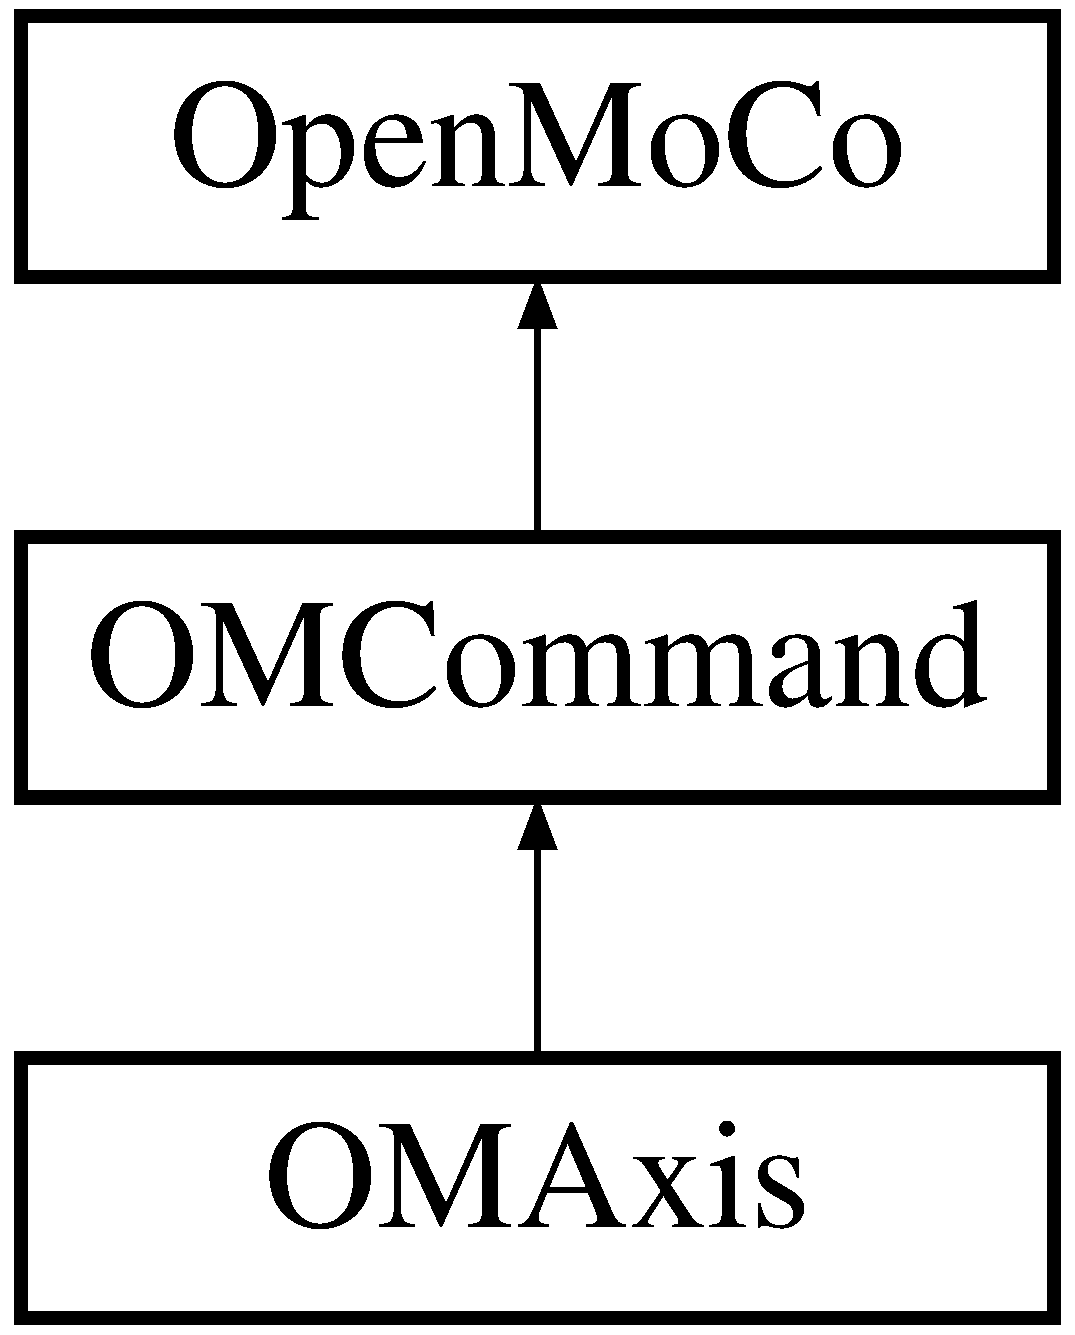
\includegraphics[height=3.000000cm]{class_o_m_axis}
\end{center}
\end{figure}
\subsection*{Public Member Functions}
\begin{DoxyCompactItemize}
\item 
\hyperlink{class_o_m_axis_a224b25d24f519b7f555c28d5f843e3c3}{OMAxis} (\hyperlink{class_o_m_controller}{OMController} $\ast$\&controller, unsigned short addr)
\end{DoxyCompactItemize}


\subsection{Constructor \& Destructor Documentation}
\hypertarget{class_o_m_axis_a224b25d24f519b7f555c28d5f843e3c3}{
\index{OMAxis@{OMAxis}!OMAxis@{OMAxis}}
\index{OMAxis@{OMAxis}!OMAxis@{OMAxis}}
\subsubsection[{OMAxis}]{\setlength{\rightskip}{0pt plus 5cm}OMAxis::OMAxis (
\begin{DoxyParamCaption}
\item[{{\bf OMController} $\ast$\&}]{controller, }
\item[{unsigned short}]{addr}
\end{DoxyParamCaption}
)\hspace{0.3cm}{\ttfamily  \mbox{[}inline\mbox{]}}}}
\label{class_o_m_axis_a224b25d24f519b7f555c28d5f843e3c3}


The documentation for this class was generated from the following file:\begin{DoxyCompactItemize}
\item 
\hyperlink{omaxis_8h}{omaxis.h}\end{DoxyCompactItemize}

\hypertarget{class_o_m_command}{
\section{OMCommand Class Reference}
\label{class_o_m_command}\index{OMCommand@{OMCommand}}
}


{\ttfamily \#include $<$omcommand.h$>$}

Inheritance diagram for OMCommand:\begin{figure}[H]
\begin{center}
\leavevmode
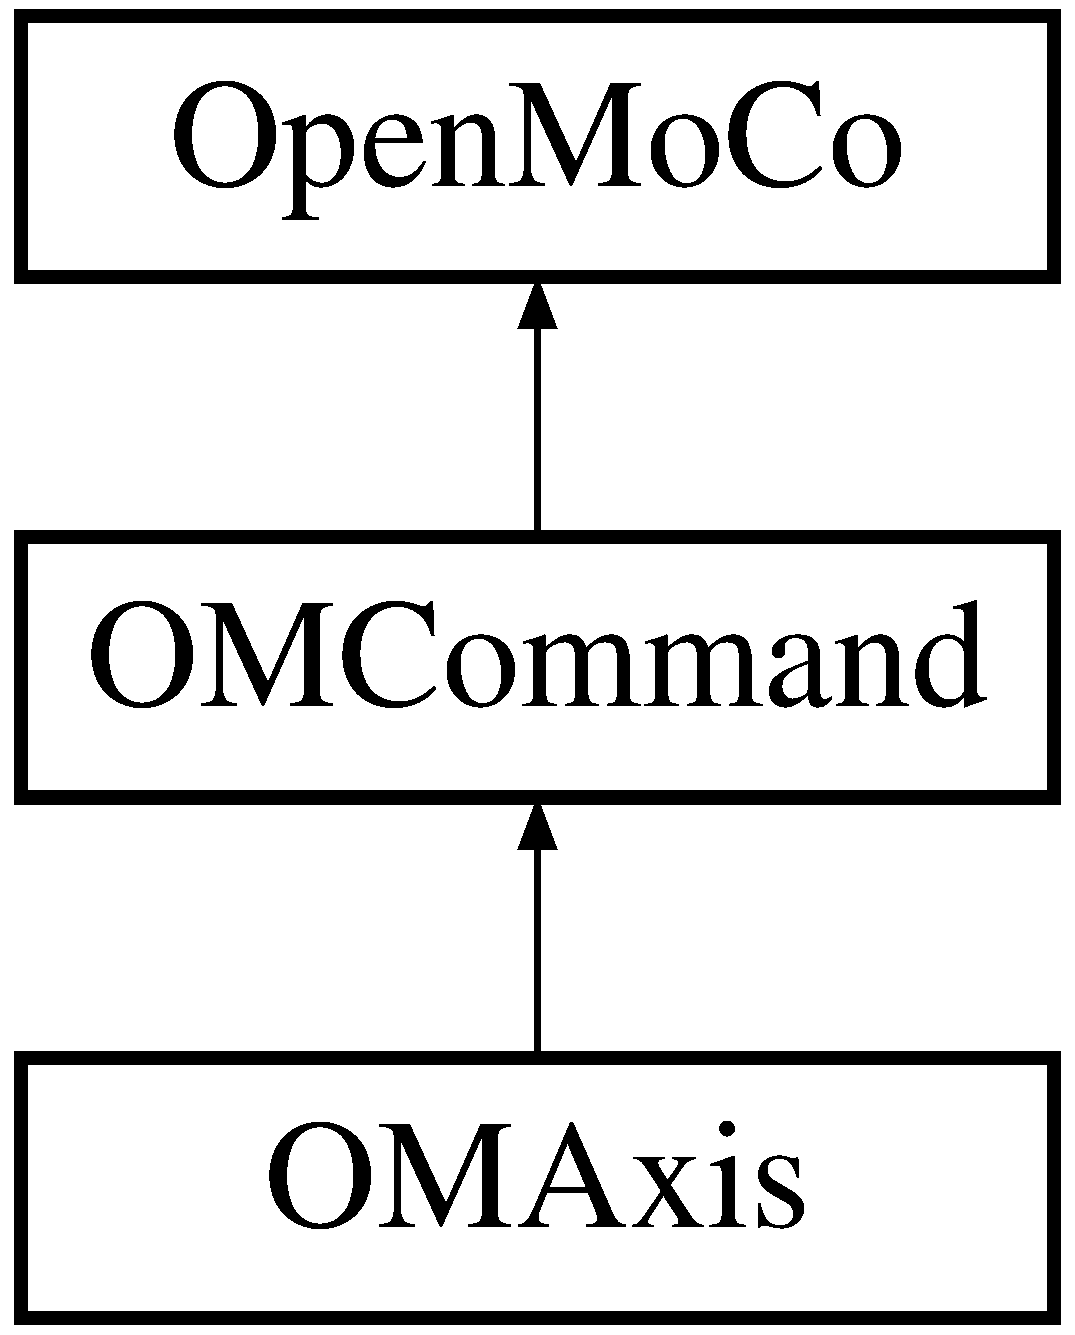
\includegraphics[height=3.000000cm]{class_o_m_command}
\end{center}
\end{figure}
\subsection*{Public Member Functions}
\begin{DoxyCompactItemize}
\item 
\hyperlink{class_o_m_command_a4309de8502be074585f5394ccca10e21}{OMCommand} (\hyperlink{class_o_m_controller}{OMController} $\ast$controller, unsigned short adr)
\item 
\hyperlink{class_o_m_command_a7dcce6f2c9f4f47d0a7eb4042c3b802c}{$\sim$OMCommand} ()
\item 
void \hyperlink{class_o_m_command_a2ad82f39f3057d972c8d65b989695888}{cameraEnable} ()
\item 
void \hyperlink{class_o_m_command_a6be90e8f9f3a6ca1bc72202b847c06b7}{cameraDisable} ()
\item 
void \hyperlink{class_o_m_command_a05f4e456e0081d9b4ebeedc7fe896dee}{play} ()
\item 
void \hyperlink{class_o_m_command_a12578b9cc0650dfc91a54e543ac1f4c8}{stop} ()
\item 
void \hyperlink{class_o_m_command_abb622e2ee5e14965011b58e1dc25a756}{pause} ()
\item 
void \hyperlink{class_o_m_command_acd98ba9e6685b63d5238f5f558f1cd0b}{home} ()
\item 
void \hyperlink{class_o_m_command_a2db56af70b4d203baba897b12fb3d931}{expose} (unsigned long)
\item 
void \hyperlink{class_o_m_command_a74794f3af8c48bc54b7dae2ac3841881}{sleep} (bool)
\item 
void \hyperlink{class_o_m_command_aa90d56c1a58c7d6b53beeae092971c84}{minAccelDelay} (unsigned short)
\item 
void \hyperlink{class_o_m_command_a15b5bc32da119b277a369d735f7a0e43}{maxAccelDelay} (unsigned short)
\item 
void \hyperlink{class_o_m_command_adc8314bfa9694ea2f1f6c1a7ed8a1fda}{rampDown} ()
\item 
void \hyperlink{class_o_m_command_a8329ee361cf2cc6214621f6ee511b97f}{debug} (bool)
\item 
void \hyperlink{class_o_m_command_a1cba427465c500cb101fd2c8173d6273}{steps} (unsigned short)
\item 
void \hyperlink{class_o_m_command_af5e4860d9cefb0c5098a70fae890fede}{rampSteps} (unsigned char)
\item 
void \hyperlink{class_o_m_command_a697e5117c035fe6af4add78396515c23}{direction} (bool)
\item 
void \hyperlink{class_o_m_command_acd5345ece18b375ba992af3b4317cb8d}{maxSteps} (unsigned long)
\item 
void \hyperlink{class_o_m_command_ac9b02c84746c59673538125ef61ae132}{interval} (unsigned short)
\item 
void \hyperlink{class_o_m_command_aab1d9a9eb29435af73c24f5799f4f8fe}{exposure} (unsigned long)
\item 
void \hyperlink{class_o_m_command_ae5a8b76a5666b1ff65216b48595932ec}{focus} (unsigned short)
\item 
void \hyperlink{class_o_m_command_aa826663213a989c75691a4c88cac4707}{maxShots} (unsigned short)
\item 
void \hyperlink{class_o_m_command_aba1bbf0fffb35a7806ed588b359e354e}{exposureDelay} (unsigned short ms)
\item 
void \hyperlink{class_o_m_command_ac674fe6db903fc35848bc10645ca36a3}{focusShutter} (bool)
\item 
void \hyperlink{class_o_m_command_ae11a454df4e3a0c756a9f9fbcd09af93}{exposureRepeat} (unsigned char)
\item 
void \hyperlink{class_o_m_command_acd64a99f15232a5946293f4f0e51a5be}{exposureRepeatAction} (unsigned char, unsigned char)
\end{DoxyCompactItemize}


\subsection{Detailed Description}
Base Command Class

Provides requisite methods for creating commands and queueing them in a specified controller. This class is not intended to be used directly, but instead through the \hyperlink{class_o_m_axis}{OMAxis} class which inherits its functions.

\begin{DoxyAuthor}{Author}
C. A. Church 
\end{DoxyAuthor}


\subsection{Constructor \& Destructor Documentation}
\hypertarget{class_o_m_command_a4309de8502be074585f5394ccca10e21}{
\index{OMCommand@{OMCommand}!OMCommand@{OMCommand}}
\index{OMCommand@{OMCommand}!OMCommand@{OMCommand}}
\subsubsection[{OMCommand}]{\setlength{\rightskip}{0pt plus 5cm}OMCommand::OMCommand (
\begin{DoxyParamCaption}
\item[{{\bf OMController} $\ast$}]{controller, }
\item[{unsigned short}]{adr}
\end{DoxyParamCaption}
)}}
\label{class_o_m_command_a4309de8502be074585f5394ccca10e21}
\hypertarget{class_o_m_command_a7dcce6f2c9f4f47d0a7eb4042c3b802c}{
\index{OMCommand@{OMCommand}!$\sim$OMCommand@{$\sim$OMCommand}}
\index{$\sim$OMCommand@{$\sim$OMCommand}!OMCommand@{OMCommand}}
\subsubsection[{$\sim$OMCommand}]{\setlength{\rightskip}{0pt plus 5cm}OMCommand::$\sim$OMCommand (
\begin{DoxyParamCaption}
{}
\end{DoxyParamCaption}
)}}
\label{class_o_m_command_a7dcce6f2c9f4f47d0a7eb4042c3b802c}


\subsection{Member Function Documentation}
\hypertarget{class_o_m_command_a6be90e8f9f3a6ca1bc72202b847c06b7}{
\index{OMCommand@{OMCommand}!cameraDisable@{cameraDisable}}
\index{cameraDisable@{cameraDisable}!OMCommand@{OMCommand}}
\subsubsection[{cameraDisable}]{\setlength{\rightskip}{0pt plus 5cm}void OMCommand::cameraDisable (
\begin{DoxyParamCaption}
{}
\end{DoxyParamCaption}
)}}
\label{class_o_m_command_a6be90e8f9f3a6ca1bc72202b847c06b7}
Disable Camera

Prevent camera from firing on cycle \hypertarget{class_o_m_command_a2ad82f39f3057d972c8d65b989695888}{
\index{OMCommand@{OMCommand}!cameraEnable@{cameraEnable}}
\index{cameraEnable@{cameraEnable}!OMCommand@{OMCommand}}
\subsubsection[{cameraEnable}]{\setlength{\rightskip}{0pt plus 5cm}void OMCommand::cameraEnable (
\begin{DoxyParamCaption}
{}
\end{DoxyParamCaption}
)}}
\label{class_o_m_command_a2ad82f39f3057d972c8d65b989695888}
Enable Camera

Enales camera, so that it will fire on cycle. \hypertarget{class_o_m_command_a8329ee361cf2cc6214621f6ee511b97f}{
\index{OMCommand@{OMCommand}!debug@{debug}}
\index{debug@{debug}!OMCommand@{OMCommand}}
\subsubsection[{debug}]{\setlength{\rightskip}{0pt plus 5cm}void OMCommand::debug (
\begin{DoxyParamCaption}
\item[{bool}]{value}
\end{DoxyParamCaption}
)}}
\label{class_o_m_command_a8329ee361cf2cc6214621f6ee511b97f}
Control Debug Line/LED

Enables or disables pulsing of the debug line/LED.


\begin{DoxyParams}{Parameters}
{\em value} & Enable (true) or disable (false) the debug line \\
\hline
\end{DoxyParams}
\hypertarget{class_o_m_command_a697e5117c035fe6af4add78396515c23}{
\index{OMCommand@{OMCommand}!direction@{direction}}
\index{direction@{direction}!OMCommand@{OMCommand}}
\subsubsection[{direction}]{\setlength{\rightskip}{0pt plus 5cm}void OMCommand::direction (
\begin{DoxyParamCaption}
\item[{bool}]{dir}
\end{DoxyParamCaption}
)}}
\label{class_o_m_command_a697e5117c035fe6af4add78396515c23}
Motor Direction

Sets the current direction


\begin{DoxyParams}{Parameters}
{\em dir} & Direction \\
\hline
\end{DoxyParams}
\hypertarget{class_o_m_command_a2db56af70b4d203baba897b12fb3d931}{
\index{OMCommand@{OMCommand}!expose@{expose}}
\index{expose@{expose}!OMCommand@{OMCommand}}
\subsubsection[{expose}]{\setlength{\rightskip}{0pt plus 5cm}void OMCommand::expose (
\begin{DoxyParamCaption}
\item[{unsigned long}]{tm}
\end{DoxyParamCaption}
)}}
\label{class_o_m_command_a2db56af70b4d203baba897b12fb3d931}
Expose Camera Now

Take an exposure immediately, even if the program is not running or the camera is disabled.


\begin{DoxyParams}{Parameters}
{\em tm} & Exposure time in milliseconds \\
\hline
\end{DoxyParams}
\hypertarget{class_o_m_command_aab1d9a9eb29435af73c24f5799f4f8fe}{
\index{OMCommand@{OMCommand}!exposure@{exposure}}
\index{exposure@{exposure}!OMCommand@{OMCommand}}
\subsubsection[{exposure}]{\setlength{\rightskip}{0pt plus 5cm}void OMCommand::exposure (
\begin{DoxyParamCaption}
\item[{unsigned long}]{ms}
\end{DoxyParamCaption}
)}}
\label{class_o_m_command_aab1d9a9eb29435af73c24f5799f4f8fe}
Exposure Time

Sets the camera exposure time (how long trigger line is held high)


\begin{DoxyParams}{Parameters}
{\em ms} & Exposure time in milliseconds \\
\hline
\end{DoxyParams}
\hypertarget{class_o_m_command_aba1bbf0fffb35a7806ed588b359e354e}{
\index{OMCommand@{OMCommand}!exposureDelay@{exposureDelay}}
\index{exposureDelay@{exposureDelay}!OMCommand@{OMCommand}}
\subsubsection[{exposureDelay}]{\setlength{\rightskip}{0pt plus 5cm}void OMCommand::exposureDelay (
\begin{DoxyParamCaption}
\item[{unsigned short}]{ms}
\end{DoxyParamCaption}
)}}
\label{class_o_m_command_aba1bbf0fffb35a7806ed588b359e354e}
Exposure Delay

Sets the camera exposure delay time (how long the program waits after the shutter has been brought high)


\begin{DoxyParams}{Parameters}
{\em ms} & Delay time in milliseconds \\
\hline
\end{DoxyParams}
\hypertarget{class_o_m_command_ae11a454df4e3a0c756a9f9fbcd09af93}{
\index{OMCommand@{OMCommand}!exposureRepeat@{exposureRepeat}}
\index{exposureRepeat@{exposureRepeat}!OMCommand@{OMCommand}}
\subsubsection[{exposureRepeat}]{\setlength{\rightskip}{0pt plus 5cm}void OMCommand::exposureRepeat (
\begin{DoxyParamCaption}
\item[{unsigned char}]{count}
\end{DoxyParamCaption}
)}}
\label{class_o_m_command_ae11a454df4e3a0c756a9f9fbcd09af93}
Camera Repeat count

Sets the camera cycle repeat count (how many photos to take per interval cycle. At each point in the interval, it will take this many photos, with each photo repeating the normal photo setting. The ability to trigger actions between each photo makes this feature more useful for gigapan and similar photo styles.)


\begin{DoxyParams}{Parameters}
{\em count} & Count of photos to take per cycle. \\
\hline
\end{DoxyParams}
\hypertarget{class_o_m_command_acd64a99f15232a5946293f4f0e51a5be}{
\index{OMCommand@{OMCommand}!exposureRepeatAction@{exposureRepeatAction}}
\index{exposureRepeatAction@{exposureRepeatAction}!OMCommand@{OMCommand}}
\subsubsection[{exposureRepeatAction}]{\setlength{\rightskip}{0pt plus 5cm}void OMCommand::exposureRepeatAction (
\begin{DoxyParamCaption}
\item[{unsigned char}]{slot, }
\item[{unsigned char}]{action}
\end{DoxyParamCaption}
)}}
\label{class_o_m_command_acd64a99f15232a5946293f4f0e51a5be}
Camera Repeat action

Sets an action id to call between each repeated exposure in an interval cycle. In this fashion, you may move motors within a cycle, rather than just between cycles. This feature is especially important in gigapanoramic shots because you may use it to quickly code in movements for grid-\/like coverage.


\begin{DoxyParams}{Parameters}
{\em slot} & \mbox{[}0..3\mbox{]} Which action slot (there are four) to add this action\\
\hline
{\em action} & Which action ID to execute \\
\hline
\end{DoxyParams}
\hypertarget{class_o_m_command_ae5a8b76a5666b1ff65216b48595932ec}{
\index{OMCommand@{OMCommand}!focus@{focus}}
\index{focus@{focus}!OMCommand@{OMCommand}}
\subsubsection[{focus}]{\setlength{\rightskip}{0pt plus 5cm}void OMCommand::focus (
\begin{DoxyParamCaption}
\item[{unsigned short}]{ms}
\end{DoxyParamCaption}
)}}
\label{class_o_m_command_ae5a8b76a5666b1ff65216b48595932ec}
Focus Tap Time

Sets the camera focus tap time (how long the focus line is held high before an exposure)


\begin{DoxyParams}{Parameters}
{\em ms} & Focus time in milliseconds \\
\hline
\end{DoxyParams}
\hypertarget{class_o_m_command_ac674fe6db903fc35848bc10645ca36a3}{
\index{OMCommand@{OMCommand}!focusShutter@{focusShutter}}
\index{focusShutter@{focusShutter}!OMCommand@{OMCommand}}
\subsubsection[{focusShutter}]{\setlength{\rightskip}{0pt plus 5cm}void OMCommand::focusShutter (
\begin{DoxyParamCaption}
\item[{bool}]{foc}
\end{DoxyParamCaption}
)}}
\label{class_o_m_command_ac674fe6db903fc35848bc10645ca36a3}
Focus with Shutter

Enables or disables connecting the focus line when the shutter line is connected. This, effectively, engages the focus whenever the shutter is engaged, as is needed with some cameras (especially Nikons).


\begin{DoxyParams}{Parameters}
{\em foc} & Enable (true) or disable (false) the focus with shutter setting \\
\hline
\end{DoxyParams}
\hypertarget{class_o_m_command_acd98ba9e6685b63d5238f5f558f1cd0b}{
\index{OMCommand@{OMCommand}!home@{home}}
\index{home@{home}!OMCommand@{OMCommand}}
\subsubsection[{home}]{\setlength{\rightskip}{0pt plus 5cm}void OMCommand::home (
\begin{DoxyParamCaption}
{}
\end{DoxyParamCaption}
)}}
\label{class_o_m_command_acd98ba9e6685b63d5238f5f558f1cd0b}
Send Motor Home

Sends motor to its set home position \hypertarget{class_o_m_command_ac9b02c84746c59673538125ef61ae132}{
\index{OMCommand@{OMCommand}!interval@{interval}}
\index{interval@{interval}!OMCommand@{OMCommand}}
\subsubsection[{interval}]{\setlength{\rightskip}{0pt plus 5cm}void OMCommand::interval (
\begin{DoxyParamCaption}
\item[{unsigned short}]{seconds}
\end{DoxyParamCaption}
)}}
\label{class_o_m_command_ac9b02c84746c59673538125ef61ae132}
Interval Seconds

Sets the camera intervalometer timing in seconds


\begin{DoxyParams}{Parameters}
{\em seconds} & Interval Seconds \\
\hline
\end{DoxyParams}
\hypertarget{class_o_m_command_a15b5bc32da119b277a369d735f7a0e43}{
\index{OMCommand@{OMCommand}!maxAccelDelay@{maxAccelDelay}}
\index{maxAccelDelay@{maxAccelDelay}!OMCommand@{OMCommand}}
\subsubsection[{maxAccelDelay}]{\setlength{\rightskip}{0pt plus 5cm}void OMCommand::maxAccelDelay (
\begin{DoxyParamCaption}
\item[{unsigned short}]{tm}
\end{DoxyParamCaption}
)}}
\label{class_o_m_command_a15b5bc32da119b277a369d735f7a0e43}
Set Max Step Delay

Specifiies Maximum Step Delay value for Acceleration.


\begin{DoxyParams}{Parameters}
{\em tm} & Microseconds of delay \\
\hline
\end{DoxyParams}
\hypertarget{class_o_m_command_aa826663213a989c75691a4c88cac4707}{
\index{OMCommand@{OMCommand}!maxShots@{maxShots}}
\index{maxShots@{maxShots}!OMCommand@{OMCommand}}
\subsubsection[{maxShots}]{\setlength{\rightskip}{0pt plus 5cm}void OMCommand::maxShots (
\begin{DoxyParamCaption}
\item[{unsigned short}]{shots}
\end{DoxyParamCaption}
)}}
\label{class_o_m_command_aa826663213a989c75691a4c88cac4707}
Max Shots

Sets the maximum \# of shots to take (program will stop when this number of shots have been taken)


\begin{DoxyParams}{Parameters}
{\em shots} & Number of shots to take \\
\hline
\end{DoxyParams}
\hypertarget{class_o_m_command_acd5345ece18b375ba992af3b4317cb8d}{
\index{OMCommand@{OMCommand}!maxSteps@{maxSteps}}
\index{maxSteps@{maxSteps}!OMCommand@{OMCommand}}
\subsubsection[{maxSteps}]{\setlength{\rightskip}{0pt plus 5cm}void OMCommand::maxSteps (
\begin{DoxyParamCaption}
\item[{unsigned long}]{stps}
\end{DoxyParamCaption}
)}}
\label{class_o_m_command_acd5345ece18b375ba992af3b4317cb8d}
Maximum Step Travel

Sets the maximum \# of steps the motor should take before stopping.


\begin{DoxyParams}{Parameters}
{\em stps} & Maximum \# of steps \\
\hline
\end{DoxyParams}
\hypertarget{class_o_m_command_aa90d56c1a58c7d6b53beeae092971c84}{
\index{OMCommand@{OMCommand}!minAccelDelay@{minAccelDelay}}
\index{minAccelDelay@{minAccelDelay}!OMCommand@{OMCommand}}
\subsubsection[{minAccelDelay}]{\setlength{\rightskip}{0pt plus 5cm}void OMCommand::minAccelDelay (
\begin{DoxyParamCaption}
\item[{unsigned short}]{tm}
\end{DoxyParamCaption}
)}}
\label{class_o_m_command_aa90d56c1a58c7d6b53beeae092971c84}
Set Min Step Delay

Specifiies Minimum Step Delay value for Acceleration.


\begin{DoxyParams}{Parameters}
{\em tm} & Microseconds of delay \\
\hline
\end{DoxyParams}
\hypertarget{class_o_m_command_abb622e2ee5e14965011b58e1dc25a756}{
\index{OMCommand@{OMCommand}!pause@{pause}}
\index{pause@{pause}!OMCommand@{OMCommand}}
\subsubsection[{pause}]{\setlength{\rightskip}{0pt plus 5cm}void OMCommand::pause (
\begin{DoxyParamCaption}
{}
\end{DoxyParamCaption}
)}}
\label{class_o_m_command_abb622e2ee5e14965011b58e1dc25a756}
Pause Program

Pause current program execution, allows starting again without loss of program information \hypertarget{class_o_m_command_a05f4e456e0081d9b4ebeedc7fe896dee}{
\index{OMCommand@{OMCommand}!play@{play}}
\index{play@{play}!OMCommand@{OMCommand}}
\subsubsection[{play}]{\setlength{\rightskip}{0pt plus 5cm}void OMCommand::play (
\begin{DoxyParamCaption}
{}
\end{DoxyParamCaption}
)}}
\label{class_o_m_command_a05f4e456e0081d9b4ebeedc7fe896dee}
Start Program

Cause program to begin playing \hypertarget{class_o_m_command_adc8314bfa9694ea2f1f6c1a7ed8a1fda}{
\index{OMCommand@{OMCommand}!rampDown@{rampDown}}
\index{rampDown@{rampDown}!OMCommand@{OMCommand}}
\subsubsection[{rampDown}]{\setlength{\rightskip}{0pt plus 5cm}void OMCommand::rampDown (
\begin{DoxyParamCaption}
{}
\end{DoxyParamCaption}
)}}
\label{class_o_m_command_adc8314bfa9694ea2f1f6c1a7ed8a1fda}
Ramp Down Now

Begin ramping down motion immediately \hypertarget{class_o_m_command_af5e4860d9cefb0c5098a70fae890fede}{
\index{OMCommand@{OMCommand}!rampSteps@{rampSteps}}
\index{rampSteps@{rampSteps}!OMCommand@{OMCommand}}
\subsubsection[{rampSteps}]{\setlength{\rightskip}{0pt plus 5cm}void OMCommand::rampSteps (
\begin{DoxyParamCaption}
\item[{unsigned char}]{cycles}
\end{DoxyParamCaption}
)}}
\label{class_o_m_command_af5e4860d9cefb0c5098a70fae890fede}
Motor Ramp Cycles

Sets the \# of shot cycles to ramp up to full speed


\begin{DoxyParams}{Parameters}
{\em cycles} & Number of cycles to accelerate over \\
\hline
\end{DoxyParams}
\hypertarget{class_o_m_command_a74794f3af8c48bc54b7dae2ac3841881}{
\index{OMCommand@{OMCommand}!sleep@{sleep}}
\index{sleep@{sleep}!OMCommand@{OMCommand}}
\subsubsection[{sleep}]{\setlength{\rightskip}{0pt plus 5cm}void OMCommand::sleep (
\begin{DoxyParamCaption}
\item[{bool}]{value}
\end{DoxyParamCaption}
)}}
\label{class_o_m_command_a74794f3af8c48bc54b7dae2ac3841881}
Control Motor Sleep

Enable or disable motor sleep between moves


\begin{DoxyParams}{Parameters}
{\em value} & Enable (true) or Disable (false) \\
\hline
\end{DoxyParams}
\hypertarget{class_o_m_command_a1cba427465c500cb101fd2c8173d6273}{
\index{OMCommand@{OMCommand}!steps@{steps}}
\index{steps@{steps}!OMCommand@{OMCommand}}
\subsubsection[{steps}]{\setlength{\rightskip}{0pt plus 5cm}void OMCommand::steps (
\begin{DoxyParamCaption}
\item[{unsigned short}]{stps}
\end{DoxyParamCaption}
)}}
\label{class_o_m_command_a1cba427465c500cb101fd2c8173d6273}
Motor Steps

Sets the \# of steps to take during each cycle


\begin{DoxyParams}{Parameters}
{\em stps} & Number of steps to take between moves \\
\hline
\end{DoxyParams}
\hypertarget{class_o_m_command_a12578b9cc0650dfc91a54e543ac1f4c8}{
\index{OMCommand@{OMCommand}!stop@{stop}}
\index{stop@{stop}!OMCommand@{OMCommand}}
\subsubsection[{stop}]{\setlength{\rightskip}{0pt plus 5cm}void OMCommand::stop (
\begin{DoxyParamCaption}
{}
\end{DoxyParamCaption}
)}}
\label{class_o_m_command_a12578b9cc0650dfc91a54e543ac1f4c8}
Stop Program

Stop program, reset back to beginning, purge state information 

The documentation for this class was generated from the following files:\begin{DoxyCompactItemize}
\item 
\hyperlink{omcommand_8h}{omcommand.h}\item 
\hyperlink{omcommand_8cpp}{omcommand.cpp}\end{DoxyCompactItemize}

\hypertarget{class_o_m_command_buffer}{
\section{OMCommandBuffer Class Reference}
\label{class_o_m_command_buffer}\index{OMCommandBuffer@{OMCommandBuffer}}
}


{\ttfamily \#include $<$omcommandbuffer.h$>$}

Inheritance diagram for OMCommandBuffer:\begin{figure}[H]
\begin{center}
\leavevmode
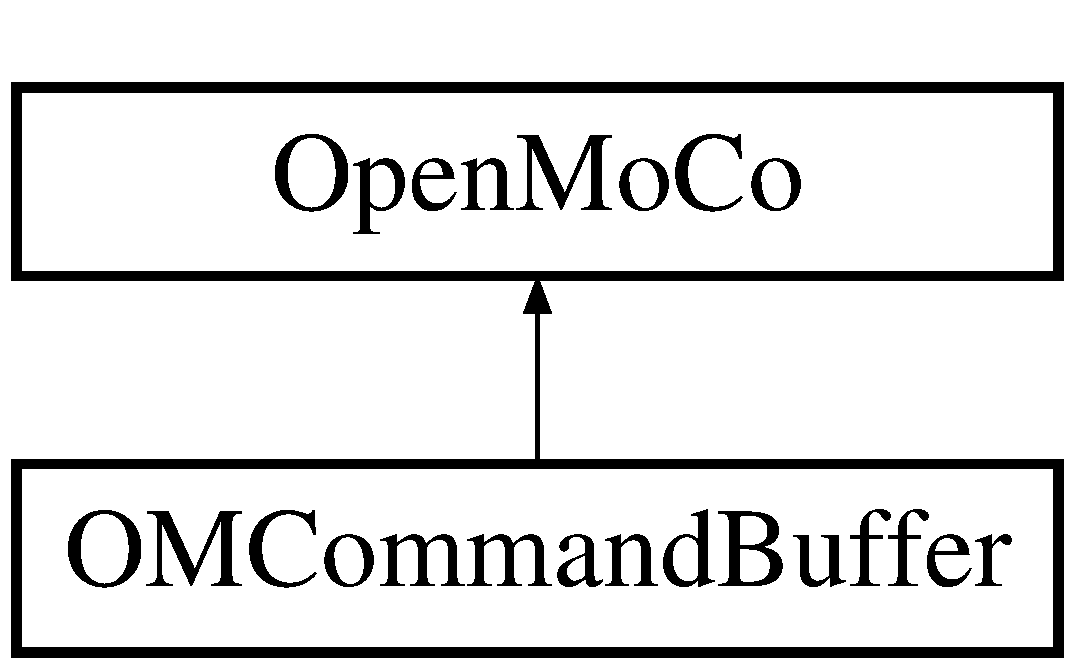
\includegraphics[height=2.000000cm]{class_o_m_command_buffer}
\end{center}
\end{figure}
\subsection*{Public Member Functions}
\begin{DoxyCompactItemize}
\item 
\hyperlink{class_o_m_command_buffer_a79bb2396d82d2eb00e8222504698189c}{OMCommandBuffer} (unsigned short addr)
\item 
\hyperlink{class_o_m_command_buffer_ae6a82bcdee2c8afe0354097313dac6f8}{$\sim$OMCommandBuffer} ()
\item 
void \hyperlink{class_o_m_command_buffer_ab23214e0ad79d0184ca105763ea165d8}{header} (char $\ast$\&, int)
\item 
void \hyperlink{class_o_m_command_buffer_a34a300d33ad70285bf490d458abb3e74}{payload} (char $\ast$\&, int)
\item 
void \hyperlink{class_o_m_command_buffer_a955f090dfece6ceef9414dce78f31d81}{setPayload} (char $\ast$\&, unsigned char, unsigned char)
\item 
unsigned int \hyperlink{class_o_m_command_buffer_a195611894a04bedb7b4637281c3e9346}{payloadSize} ()
\item 
unsigned int \hyperlink{class_o_m_command_buffer_aa30260f093bb3a5d2aa9ffe5617f1503}{headerSize} ()
\end{DoxyCompactItemize}
\subsection*{Static Public Attributes}
\begin{DoxyCompactItemize}
\item 
static const int \hyperlink{class_o_m_command_buffer_a529b47966a6c91743ea5e4f1d584b1f2}{errOutOfMemory} = 3
\end{DoxyCompactItemize}


\subsection{Detailed Description}
Create a buffer representing the parts of an \hyperlink{class_open_mo_co}{OpenMoCo} Engine command

Provides requisite methods for packaging and transporting a command to be sent to a controller (or read from a controller) and managed through the controller queue. This class is not intended to be used directly, but instead is leveraged by the \hyperlink{class_o_m_axis}{OMAxis}, \hyperlink{class_o_m_command}{OMCommand}, and \hyperlink{class_o_m_controller}{OMController} classes. You should not be creating \hyperlink{class_o_m_command_buffer}{OMCommandBuffer} or \hyperlink{class_o_m_command}{OMCommand} objects directly, but should be interacting with the \hyperlink{class_o_m_axis}{OMAxis} and \hyperlink{class_o_m_controller}{OMController} classes only.

\begin{DoxyAuthor}{Author}
C. A. Church 
\end{DoxyAuthor}


\subsection{Constructor \& Destructor Documentation}
\hypertarget{class_o_m_command_buffer_a79bb2396d82d2eb00e8222504698189c}{
\index{OMCommandBuffer@{OMCommandBuffer}!OMCommandBuffer@{OMCommandBuffer}}
\index{OMCommandBuffer@{OMCommandBuffer}!OMCommandBuffer@{OMCommandBuffer}}
\subsubsection[{OMCommandBuffer}]{\setlength{\rightskip}{0pt plus 5cm}OMCommandBuffer::OMCommandBuffer (
\begin{DoxyParamCaption}
\item[{unsigned short}]{addr}
\end{DoxyParamCaption}
)}}
\label{class_o_m_command_buffer_a79bb2396d82d2eb00e8222504698189c}
A char buffer containing the elements of an OMTLE Command

Create a new instance of the \hyperlink{class_o_m_command_buffer}{OMCommandBuffer} object, which holds the parts of an OMTLE command, such that it can be sent to a communication handler.


\begin{DoxyParams}{Parameters}
{\em addr} & Address of the device which we will be speaking to \\
\hline
\end{DoxyParams}
\hypertarget{class_o_m_command_buffer_ae6a82bcdee2c8afe0354097313dac6f8}{
\index{OMCommandBuffer@{OMCommandBuffer}!$\sim$OMCommandBuffer@{$\sim$OMCommandBuffer}}
\index{$\sim$OMCommandBuffer@{$\sim$OMCommandBuffer}!OMCommandBuffer@{OMCommandBuffer}}
\subsubsection[{$\sim$OMCommandBuffer}]{\setlength{\rightskip}{0pt plus 5cm}OMCommandBuffer::$\sim$OMCommandBuffer (
\begin{DoxyParamCaption}
{}
\end{DoxyParamCaption}
)}}
\label{class_o_m_command_buffer_ae6a82bcdee2c8afe0354097313dac6f8}


\subsection{Member Function Documentation}
\hypertarget{class_o_m_command_buffer_ab23214e0ad79d0184ca105763ea165d8}{
\index{OMCommandBuffer@{OMCommandBuffer}!header@{header}}
\index{header@{header}!OMCommandBuffer@{OMCommandBuffer}}
\subsubsection[{header}]{\setlength{\rightskip}{0pt plus 5cm}void OMCommandBuffer::header (
\begin{DoxyParamCaption}
\item[{char $\ast$\&}]{rdBuf, }
\item[{int}]{len}
\end{DoxyParamCaption}
)}}
\label{class_o_m_command_buffer_ab23214e0ad79d0184ca105763ea165d8}
Retrieves the header section of the command

Copies the header of the command sequence into a specified character buffer. You must specify a length of bytes to be copied, and if you specify fewer bytes than the header has, the specified length of bytes from your buffer will be over-\/ written with the matching bytes from the header section.


\begin{DoxyParams}{Parameters}
{\em rdBuf} & A charcter pointer, with enough memory allocated to hold the specified number of bytes.\\
\hline
{\em len} & The length of bytes of the header to copy into the buffer \\
\hline
\end{DoxyParams}
\hypertarget{class_o_m_command_buffer_aa30260f093bb3a5d2aa9ffe5617f1503}{
\index{OMCommandBuffer@{OMCommandBuffer}!headerSize@{headerSize}}
\index{headerSize@{headerSize}!OMCommandBuffer@{OMCommandBuffer}}
\subsubsection[{headerSize}]{\setlength{\rightskip}{0pt plus 5cm}unsigned int OMCommandBuffer::headerSize (
\begin{DoxyParamCaption}
{}
\end{DoxyParamCaption}
)}}
\label{class_o_m_command_buffer_aa30260f093bb3a5d2aa9ffe5617f1503}
Retrieves the size of the header.

Retrieves the size, in bytes, of the header.

\begin{DoxyReturn}{Returns}
the size of the header, in bytes. 
\end{DoxyReturn}
\hypertarget{class_o_m_command_buffer_a34a300d33ad70285bf490d458abb3e74}{
\index{OMCommandBuffer@{OMCommandBuffer}!payload@{payload}}
\index{payload@{payload}!OMCommandBuffer@{OMCommandBuffer}}
\subsubsection[{payload}]{\setlength{\rightskip}{0pt plus 5cm}void OMCommandBuffer::payload (
\begin{DoxyParamCaption}
\item[{char $\ast$\&}]{rdBuf, }
\item[{int}]{len}
\end{DoxyParamCaption}
)}}
\label{class_o_m_command_buffer_a34a300d33ad70285bf490d458abb3e74}
Retrieves the payload section of the command.

Copies the payload of the command sequence into a specified character buffer. You must specify a length of bytes to be copied, and if you specify fewer bytes than the payload has, the specified length of bytes from your buffer will be over-\/ written with the matching bytes from the payload section.


\begin{DoxyParams}{Parameters}
{\em rdBuf} & A charcter pointer, with enough memory allocated to hold the specified number of bytes.\\
\hline
{\em len} & The length of bytes of the payload to overwrite in the buffer \\
\hline
\end{DoxyParams}
\hypertarget{class_o_m_command_buffer_a195611894a04bedb7b4637281c3e9346}{
\index{OMCommandBuffer@{OMCommandBuffer}!payloadSize@{payloadSize}}
\index{payloadSize@{payloadSize}!OMCommandBuffer@{OMCommandBuffer}}
\subsubsection[{payloadSize}]{\setlength{\rightskip}{0pt plus 5cm}unsigned int OMCommandBuffer::payloadSize (
\begin{DoxyParamCaption}
{}
\end{DoxyParamCaption}
)}}
\label{class_o_m_command_buffer_a195611894a04bedb7b4637281c3e9346}
Retrieves the size of the payload.

Retrieves the size, in bytes, of the payload.

\begin{DoxyReturn}{Returns}
the size of the payload, in bytes. 
\end{DoxyReturn}
\hypertarget{class_o_m_command_buffer_a955f090dfece6ceef9414dce78f31d81}{
\index{OMCommandBuffer@{OMCommandBuffer}!setPayload@{setPayload}}
\index{setPayload@{setPayload}!OMCommandBuffer@{OMCommandBuffer}}
\subsubsection[{setPayload}]{\setlength{\rightskip}{0pt plus 5cm}void OMCommandBuffer::setPayload (
\begin{DoxyParamCaption}
\item[{char $\ast$\&}]{buf, }
\item[{unsigned char}]{cmd, }
\item[{unsigned char}]{len}
\end{DoxyParamCaption}
)}}
\label{class_o_m_command_buffer_a955f090dfece6ceef9414dce78f31d81}
Specify the payload contents.

Adds the command payload to the object.


\begin{DoxyParams}{Parameters}
{\em buf} & Payload data\\
\hline
{\em cmd} & Primary command\\
\hline
{\em len} & Command Data Length \\
\hline
\end{DoxyParams}


\subsection{Member Data Documentation}
\hypertarget{class_o_m_command_buffer_a529b47966a6c91743ea5e4f1d584b1f2}{
\index{OMCommandBuffer@{OMCommandBuffer}!errOutOfMemory@{errOutOfMemory}}
\index{errOutOfMemory@{errOutOfMemory}!OMCommandBuffer@{OMCommandBuffer}}
\subsubsection[{errOutOfMemory}]{\setlength{\rightskip}{0pt plus 5cm}const int {\bf OMCommandBuffer::errOutOfMemory} = 3\hspace{0.3cm}{\ttfamily  \mbox{[}static\mbox{]}}}}
\label{class_o_m_command_buffer_a529b47966a6c91743ea5e4f1d584b1f2}


Reimplemented from \hyperlink{class_open_mo_co_a0b6b40784caadf923e620295b47d6c39}{OpenMoCo}.



The documentation for this class was generated from the following files:\begin{DoxyCompactItemize}
\item 
\hyperlink{omcommandbuffer_8h}{omcommandbuffer.h}\item 
\hyperlink{omcommandbuffer_8cpp}{omcommandbuffer.cpp}\end{DoxyCompactItemize}

\hypertarget{class_o_m_controller}{
\section{OMController Class Reference}
\label{class_o_m_controller}\index{OMController@{OMController}}
}


{\ttfamily \#include $<$omcontroller.h$>$}

Inheritance diagram for OMController:\begin{figure}[H]
\begin{center}
\leavevmode
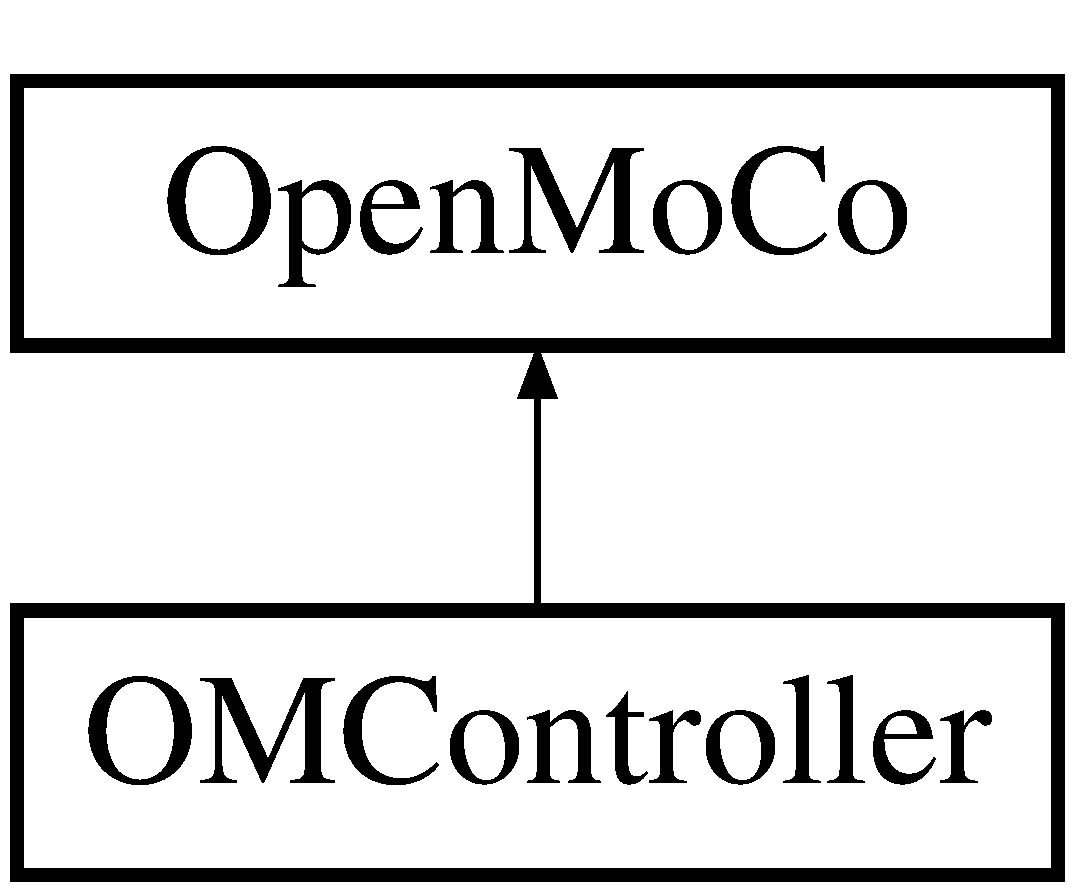
\includegraphics[height=2.000000cm]{class_o_m_controller}
\end{center}
\end{figure}
\subsection*{Signals}
\begin{DoxyCompactItemize}
\item 
void \hyperlink{class_o_m_controller_a16a02fca40829bb599649af820b59dec}{commandQueued} (\hyperlink{class_o_m_command_buffer}{OMCommandBuffer} $\ast$)
\end{DoxyCompactItemize}
\subsection*{Public Member Functions}
\begin{DoxyCompactItemize}
\item 
\hyperlink{class_o_m_controller_a37eb41ecd6775bd52ed520de69791ee5}{OMController} (char $\ast$)
\item 
\hyperlink{class_o_m_controller_a47ede74e236098c8b6f99c3de09f83b2}{$\sim$OMController} ()
\item 
\hyperlink{class_o_m_controller_a3480c3c367380bcea66825aae681c5c2}{OMController} (const \hyperlink{class_o_m_controller}{OMController} \&)
\item 
void \hyperlink{class_o_m_controller_a6cd9727f3c24525d0fa2903f59c4f2d9}{queueCommand} (\hyperlink{class_o_m_command_buffer}{OMCommandBuffer} $\ast$\&cmdBuf)
\item 
void \hyperlink{class_o_m_controller_a1e175037d84423402c04f73bc913f735}{connect} ()
\end{DoxyCompactItemize}


\subsection{Constructor \& Destructor Documentation}
\hypertarget{class_o_m_controller_a37eb41ecd6775bd52ed520de69791ee5}{
\index{OMController@{OMController}!OMController@{OMController}}
\index{OMController@{OMController}!OMController@{OMController}}
\subsubsection[{OMController}]{\setlength{\rightskip}{0pt plus 5cm}OMController::OMController (
\begin{DoxyParamCaption}
\item[{char $\ast$}]{port}
\end{DoxyParamCaption}
)}}
\label{class_o_m_controller_a37eb41ecd6775bd52ed520de69791ee5}
Constructs a new Controller

Create a new controller, attached to a particular port. You must also specify the buffer size for commands waiting to go out.


\begin{DoxyParams}{Parameters}
{\em port} & The serial port name \\
\hline
\end{DoxyParams}
\hypertarget{class_o_m_controller_a47ede74e236098c8b6f99c3de09f83b2}{
\index{OMController@{OMController}!$\sim$OMController@{$\sim$OMController}}
\index{$\sim$OMController@{$\sim$OMController}!OMController@{OMController}}
\subsubsection[{$\sim$OMController}]{\setlength{\rightskip}{0pt plus 5cm}OMController::$\sim$OMController (
\begin{DoxyParamCaption}
{}
\end{DoxyParamCaption}
)}}
\label{class_o_m_controller_a47ede74e236098c8b6f99c3de09f83b2}
\hypertarget{class_o_m_controller_a3480c3c367380bcea66825aae681c5c2}{
\index{OMController@{OMController}!OMController@{OMController}}
\index{OMController@{OMController}!OMController@{OMController}}
\subsubsection[{OMController}]{\setlength{\rightskip}{0pt plus 5cm}OMController::OMController (
\begin{DoxyParamCaption}
\item[{const {\bf OMController} \&}]{}
\end{DoxyParamCaption}
)\hspace{0.3cm}{\ttfamily  \mbox{[}inline\mbox{]}}}}
\label{class_o_m_controller_a3480c3c367380bcea66825aae681c5c2}


\subsection{Member Function Documentation}
\hypertarget{class_o_m_controller_a16a02fca40829bb599649af820b59dec}{
\index{OMController@{OMController}!commandQueued@{commandQueued}}
\index{commandQueued@{commandQueued}!OMController@{OMController}}
\subsubsection[{commandQueued}]{\setlength{\rightskip}{0pt plus 5cm}void OMController::commandQueued (
\begin{DoxyParamCaption}
\item[{{\bf OMCommandBuffer} $\ast$}]{}
\end{DoxyParamCaption}
)\hspace{0.3cm}{\ttfamily  \mbox{[}signal\mbox{]}}}}
\label{class_o_m_controller_a16a02fca40829bb599649af820b59dec}
\hypertarget{class_o_m_controller_a1e175037d84423402c04f73bc913f735}{
\index{OMController@{OMController}!connect@{connect}}
\index{connect@{connect}!OMController@{OMController}}
\subsubsection[{connect}]{\setlength{\rightskip}{0pt plus 5cm}void OMController::connect (
\begin{DoxyParamCaption}
{}
\end{DoxyParamCaption}
)}}
\label{class_o_m_controller_a1e175037d84423402c04f73bc913f735}
Connect to the specified serial port

Opens the configured serial device


\begin{DoxyExceptions}{Exceptions}
{\em errSerialNotAvailable} & Serial connection was unavailable. \\
\hline
\end{DoxyExceptions}
\hypertarget{class_o_m_controller_a6cd9727f3c24525d0fa2903f59c4f2d9}{
\index{OMController@{OMController}!queueCommand@{queueCommand}}
\index{queueCommand@{queueCommand}!OMController@{OMController}}
\subsubsection[{queueCommand}]{\setlength{\rightskip}{0pt plus 5cm}void OMController::queueCommand (
\begin{DoxyParamCaption}
\item[{{\bf OMCommandBuffer} $\ast$\&}]{cmdBuf}
\end{DoxyParamCaption}
)}}
\label{class_o_m_controller_a6cd9727f3c24525d0fa2903f59c4f2d9}
Adds a command to the command queue


\begin{DoxyParams}{Parameters}
{\em cmdBuf} & The address of a properly created (i.e. payload set) \hyperlink{class_o_m_command_buffer}{OMCommandBuffer} object pointer \\
\hline
\end{DoxyParams}


The documentation for this class was generated from the following files:\begin{DoxyCompactItemize}
\item 
\hyperlink{omcontroller_8h}{omcontroller.h}\item 
\hyperlink{omcontroller_8cpp}{omcontroller.cpp}\end{DoxyCompactItemize}

\hypertarget{class_o_m_serial_mgr}{
\section{OMSerialMgr Class Reference}
\label{class_o_m_serial_mgr}\index{OMSerialMgr@{OMSerialMgr}}
}


{\ttfamily \#include $<$omserialmgr.h$>$}

Inheritance diagram for OMSerialMgr:\begin{figure}[H]
\begin{center}
\leavevmode
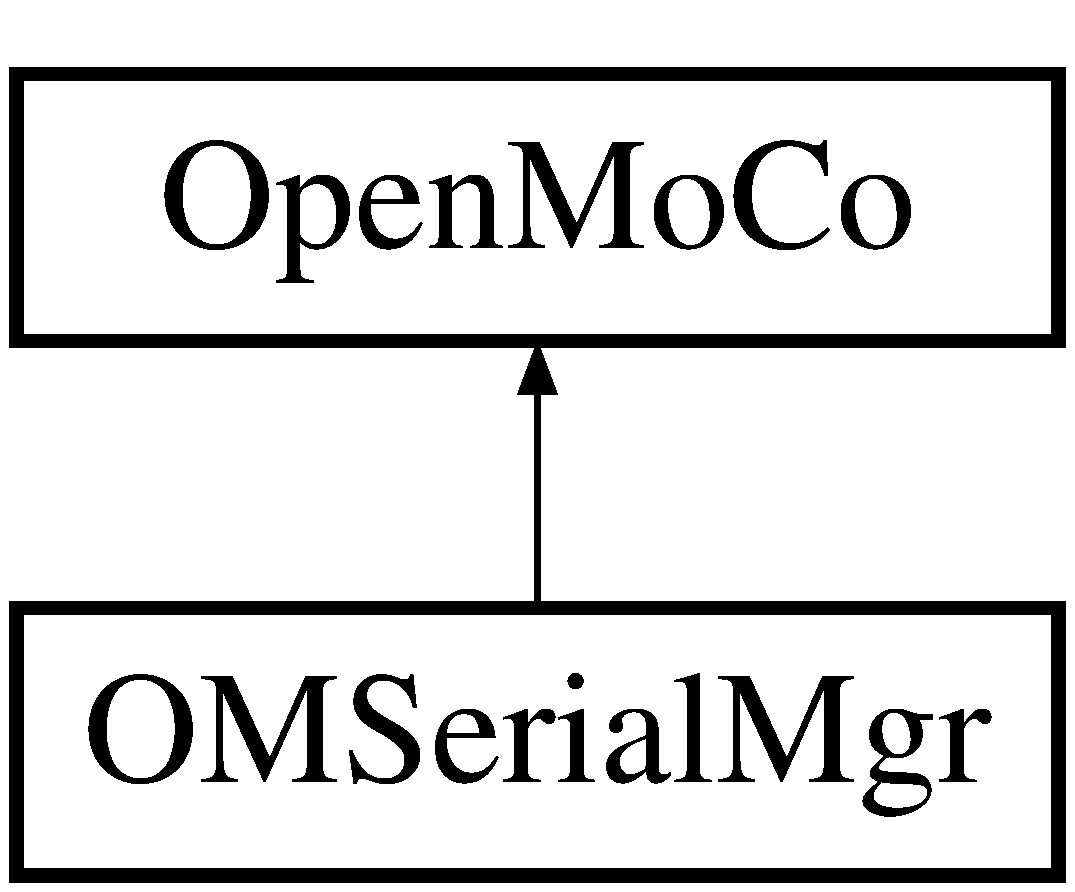
\includegraphics[height=2.000000cm]{class_o_m_serial_mgr}
\end{center}
\end{figure}
\subsection*{Public Slots}
\begin{DoxyCompactItemize}
\item 
void \hyperlink{class_o_m_serial_mgr_af4cad4cb9f1a51d4c843f7b2da2ed438}{commandAdded} (\hyperlink{class_o_m_command_buffer}{OMCommandBuffer} $\ast$)
\end{DoxyCompactItemize}
\subsection*{Signals}
\begin{DoxyCompactItemize}
\item 
void \hyperlink{class_o_m_serial_mgr_a12dd6030d34fb0b5ec83b9fd5adda481}{commandComplete} (\hyperlink{class_o_m_command_buffer}{OMCommandBuffer} $\ast$)
\end{DoxyCompactItemize}
\subsection*{Public Member Functions}
\begin{DoxyCompactItemize}
\item 
\hyperlink{class_o_m_serial_mgr_aaf3e717e0d05702a9490845d146718a6}{OMSerialMgr} (char $\ast$)
\item 
void \hyperlink{class_o_m_serial_mgr_ab1939185db07f5fb4cf73819c776384d}{connect} ()
\item 
void \hyperlink{class_o_m_serial_mgr_aeb0015e25ab9758c1db5c374a2c84612}{run} ()
\end{DoxyCompactItemize}


\subsection{Constructor \& Destructor Documentation}
\hypertarget{class_o_m_serial_mgr_aaf3e717e0d05702a9490845d146718a6}{
\index{OMSerialMgr@{OMSerialMgr}!OMSerialMgr@{OMSerialMgr}}
\index{OMSerialMgr@{OMSerialMgr}!OMSerialMgr@{OMSerialMgr}}
\subsubsection[{OMSerialMgr}]{\setlength{\rightskip}{0pt plus 5cm}OMSerialMgr::OMSerialMgr (
\begin{DoxyParamCaption}
\item[{char $\ast$}]{port}
\end{DoxyParamCaption}
)}}
\label{class_o_m_serial_mgr_aaf3e717e0d05702a9490845d146718a6}
\hyperlink{class_open_mo_co}{OpenMoCo} Serial Manager

Create a new serial manager for a serial port. Creates a new serial object and a thread to manage messages being sent to and from that serial object.


\begin{DoxyParams}{Parameters}
{\em port} & The serial port name \\
\hline
\end{DoxyParams}


\subsection{Member Function Documentation}
\hypertarget{class_o_m_serial_mgr_af4cad4cb9f1a51d4c843f7b2da2ed438}{
\index{OMSerialMgr@{OMSerialMgr}!commandAdded@{commandAdded}}
\index{commandAdded@{commandAdded}!OMSerialMgr@{OMSerialMgr}}
\subsubsection[{commandAdded}]{\setlength{\rightskip}{0pt plus 5cm}void OMSerialMgr::commandAdded (
\begin{DoxyParamCaption}
\item[{{\bf OMCommandBuffer} $\ast$}]{thsCmd}
\end{DoxyParamCaption}
)\hspace{0.3cm}{\ttfamily  \mbox{[}slot\mbox{]}}}}
\label{class_o_m_serial_mgr_af4cad4cb9f1a51d4c843f7b2da2ed438}
Command Entry Slot

Issue a command to the serial device


\begin{DoxyParams}{Parameters}
{\em thsCmd} & The command buffer to be sent \\
\hline
\end{DoxyParams}
\hypertarget{class_o_m_serial_mgr_a12dd6030d34fb0b5ec83b9fd5adda481}{
\index{OMSerialMgr@{OMSerialMgr}!commandComplete@{commandComplete}}
\index{commandComplete@{commandComplete}!OMSerialMgr@{OMSerialMgr}}
\subsubsection[{commandComplete}]{\setlength{\rightskip}{0pt plus 5cm}void OMSerialMgr::commandComplete (
\begin{DoxyParamCaption}
\item[{{\bf OMCommandBuffer} $\ast$}]{}
\end{DoxyParamCaption}
)\hspace{0.3cm}{\ttfamily  \mbox{[}signal\mbox{]}}}}
\label{class_o_m_serial_mgr_a12dd6030d34fb0b5ec83b9fd5adda481}
\hypertarget{class_o_m_serial_mgr_ab1939185db07f5fb4cf73819c776384d}{
\index{OMSerialMgr@{OMSerialMgr}!connect@{connect}}
\index{connect@{connect}!OMSerialMgr@{OMSerialMgr}}
\subsubsection[{connect}]{\setlength{\rightskip}{0pt plus 5cm}void OMSerialMgr::connect (
\begin{DoxyParamCaption}
{}
\end{DoxyParamCaption}
)}}
\label{class_o_m_serial_mgr_ab1939185db07f5fb4cf73819c776384d}
Connect to serial device

Initiates serial connection.


\begin{DoxyExceptions}{Exceptions}
{\em errSerialNotAvailable} & The serial port could not be opened. \\
\hline
\end{DoxyExceptions}
\hypertarget{class_o_m_serial_mgr_aeb0015e25ab9758c1db5c374a2c84612}{
\index{OMSerialMgr@{OMSerialMgr}!run@{run}}
\index{run@{run}!OMSerialMgr@{OMSerialMgr}}
\subsubsection[{run}]{\setlength{\rightskip}{0pt plus 5cm}void OMSerialMgr::run (
\begin{DoxyParamCaption}
{}
\end{DoxyParamCaption}
)}}
\label{class_o_m_serial_mgr_aeb0015e25ab9758c1db5c374a2c84612}


The documentation for this class was generated from the following files:\begin{DoxyCompactItemize}
\item 
\hyperlink{omserialmgr_8h}{omserialmgr.h}\item 
\hyperlink{omserialmgr_8cpp}{omserialmgr.cpp}\end{DoxyCompactItemize}

\hypertarget{class_open_mo_co}{
\section{OpenMoCo Class Reference}
\label{class_open_mo_co}\index{OpenMoCo@{OpenMoCo}}
}


{\ttfamily \#include $<$openmoco.h$>$}

Inheritance diagram for OpenMoCo:\begin{figure}[H]
\begin{center}
\leavevmode
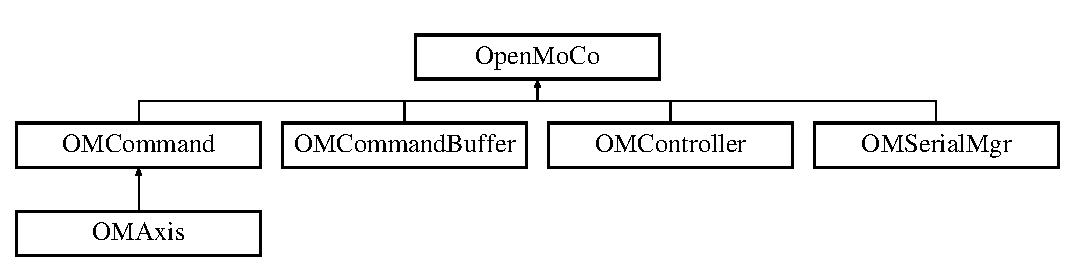
\includegraphics[height=3.000000cm]{class_open_mo_co}
\end{center}
\end{figure}
\subsection*{Public Member Functions}
\begin{DoxyCompactItemize}
\item 
\hyperlink{class_open_mo_co_a85877da7663732c3f2320d96df47d198}{OpenMoCo} ()
\end{DoxyCompactItemize}
\subsection*{Static Public Attributes}
\begin{DoxyCompactItemize}
\item 
static const int \hyperlink{class_open_mo_co_aa00b35926b1595d53734089ecb5cf240}{errInvalidArgument} = 2
\item 
static const int \hyperlink{class_open_mo_co_a0b6b40784caadf923e620295b47d6c39}{errOutOfMemory} = 3
\item 
static const int \hyperlink{class_open_mo_co_aa4c6578fae22829f8270eea20e002a79}{notQueued} = 4
\item 
static const int \hyperlink{class_open_mo_co_ad444289e4c29d2c419b232e8de1ab5e7}{errSerialNotAvailable} = 5
\end{DoxyCompactItemize}


\subsection{Constructor \& Destructor Documentation}
\hypertarget{class_open_mo_co_a85877da7663732c3f2320d96df47d198}{
\index{OpenMoCo@{OpenMoCo}!OpenMoCo@{OpenMoCo}}
\index{OpenMoCo@{OpenMoCo}!OpenMoCo@{OpenMoCo}}
\subsubsection[{OpenMoCo}]{\setlength{\rightskip}{0pt plus 5cm}OpenMoCo::OpenMoCo (
\begin{DoxyParamCaption}
{}
\end{DoxyParamCaption}
)}}
\label{class_open_mo_co_a85877da7663732c3f2320d96df47d198}


\subsection{Member Data Documentation}
\hypertarget{class_open_mo_co_aa00b35926b1595d53734089ecb5cf240}{
\index{OpenMoCo@{OpenMoCo}!errInvalidArgument@{errInvalidArgument}}
\index{errInvalidArgument@{errInvalidArgument}!OpenMoCo@{OpenMoCo}}
\subsubsection[{errInvalidArgument}]{\setlength{\rightskip}{0pt plus 5cm}const int {\bf OpenMoCo::errInvalidArgument} = 2\hspace{0.3cm}{\ttfamily  \mbox{[}static\mbox{]}}}}
\label{class_open_mo_co_aa00b35926b1595d53734089ecb5cf240}
\hypertarget{class_open_mo_co_a0b6b40784caadf923e620295b47d6c39}{
\index{OpenMoCo@{OpenMoCo}!errOutOfMemory@{errOutOfMemory}}
\index{errOutOfMemory@{errOutOfMemory}!OpenMoCo@{OpenMoCo}}
\subsubsection[{errOutOfMemory}]{\setlength{\rightskip}{0pt plus 5cm}const int {\bf OpenMoCo::errOutOfMemory} = 3\hspace{0.3cm}{\ttfamily  \mbox{[}static\mbox{]}}}}
\label{class_open_mo_co_a0b6b40784caadf923e620295b47d6c39}


Reimplemented in \hyperlink{class_o_m_command_buffer_a529b47966a6c91743ea5e4f1d584b1f2}{OMCommandBuffer}.

\hypertarget{class_open_mo_co_ad444289e4c29d2c419b232e8de1ab5e7}{
\index{OpenMoCo@{OpenMoCo}!errSerialNotAvailable@{errSerialNotAvailable}}
\index{errSerialNotAvailable@{errSerialNotAvailable}!OpenMoCo@{OpenMoCo}}
\subsubsection[{errSerialNotAvailable}]{\setlength{\rightskip}{0pt plus 5cm}const int {\bf OpenMoCo::errSerialNotAvailable} = 5\hspace{0.3cm}{\ttfamily  \mbox{[}static\mbox{]}}}}
\label{class_open_mo_co_ad444289e4c29d2c419b232e8de1ab5e7}
\hypertarget{class_open_mo_co_aa4c6578fae22829f8270eea20e002a79}{
\index{OpenMoCo@{OpenMoCo}!notQueued@{notQueued}}
\index{notQueued@{notQueued}!OpenMoCo@{OpenMoCo}}
\subsubsection[{notQueued}]{\setlength{\rightskip}{0pt plus 5cm}const int {\bf OpenMoCo::notQueued} = 4\hspace{0.3cm}{\ttfamily  \mbox{[}static\mbox{]}}}}
\label{class_open_mo_co_aa4c6578fae22829f8270eea20e002a79}


The documentation for this class was generated from the following files:\begin{DoxyCompactItemize}
\item 
\hyperlink{openmoco_8h}{openmoco.h}\item 
\hyperlink{openmoco_8cpp}{openmoco.cpp}\end{DoxyCompactItemize}

\chapter{File Documentation}
\hypertarget{main_8cpp}{
\section{main.cpp File Reference}
\label{main_8cpp}\index{main.cpp@{main.cpp}}
}
{\ttfamily \#include $<$QtGui/QApplication$>$}\par
{\ttfamily \#include $<$QDebug$>$}\par
{\ttfamily \#include \char`\"{}mainwindow.h\char`\"{}}\par
{\ttfamily \#include \char`\"{}omcommand.h\char`\"{}}\par
{\ttfamily \#include \char`\"{}omcontroller.h\char`\"{}}\par
{\ttfamily \#include \char`\"{}omaxis.h\char`\"{}}\par
\subsection*{Functions}
\begin{DoxyCompactItemize}
\item 
int \hyperlink{main_8cpp_a0ddf1224851353fc92bfbff6f499fa97}{main} (int argc, char $\ast$argv\mbox{[}$\,$\mbox{]})
\end{DoxyCompactItemize}


\subsection{Function Documentation}
\hypertarget{main_8cpp_a0ddf1224851353fc92bfbff6f499fa97}{
\index{main.cpp@{main.cpp}!main@{main}}
\index{main@{main}!main.cpp@{main.cpp}}
\subsubsection[{main}]{\setlength{\rightskip}{0pt plus 5cm}int main (
\begin{DoxyParamCaption}
\item[{int}]{argc, }
\item[{char $\ast$}]{argv\mbox{[}$\,$\mbox{]}}
\end{DoxyParamCaption}
)}}
\label{main_8cpp_a0ddf1224851353fc92bfbff6f499fa97}

\hypertarget{mainwindow_8cpp}{
\section{mainwindow.cpp File Reference}
\label{mainwindow_8cpp}\index{mainwindow.cpp@{mainwindow.cpp}}
}
{\ttfamily \#include \char`\"{}mainwindow.h\char`\"{}}\par
{\ttfamily \#include \char`\"{}ui\_\-mainwindow.h\char`\"{}}\par

\hypertarget{mainwindow_8h}{
\section{mainwindow.h File Reference}
\label{mainwindow_8h}\index{mainwindow.h@{mainwindow.h}}
}
{\ttfamily \#include $<$QMainWindow$>$}\par
\subsection*{Classes}
\begin{DoxyCompactItemize}
\item 
class \hyperlink{class_main_window}{MainWindow}
\end{DoxyCompactItemize}
\subsection*{Namespaces}
\begin{DoxyCompactItemize}
\item 
namespace \hyperlink{namespace_ui}{Ui}
\end{DoxyCompactItemize}

\hypertarget{omaxis_8cpp}{
\section{omaxis.cpp File Reference}
\label{omaxis_8cpp}\index{omaxis.cpp@{omaxis.cpp}}
}
{\ttfamily \#include \char`\"{}omaxis.h\char`\"{}}\par

\hypertarget{omaxis_8h}{
\section{omaxis.h File Reference}
\label{omaxis_8h}\index{omaxis.h@{omaxis.h}}
}
{\ttfamily \#include \char`\"{}omcommand.h\char`\"{}}\par
\subsection*{Classes}
\begin{DoxyCompactItemize}
\item 
class \hyperlink{class_o_m_axis}{OMAxis}
\end{DoxyCompactItemize}

\hypertarget{omcommand_8cpp}{
\section{omcommand.cpp File Reference}
\label{omcommand_8cpp}\index{omcommand.cpp@{omcommand.cpp}}
}
{\ttfamily \#include $<$stdlib.h$>$}\par
{\ttfamily \#include $<$stdio.h$>$}\par
{\ttfamily \#include $<$string.h$>$}\par
{\ttfamily \#include $<$QDebug$>$}\par
{\ttfamily \#include \char`\"{}omcommand.h\char`\"{}}\par

\hypertarget{omcommand_8h}{
\section{omcommand.h File Reference}
\label{omcommand_8h}\index{omcommand.h@{omcommand.h}}
}
{\ttfamily \#include \char`\"{}omcommandbuffer.h\char`\"{}}\par
{\ttfamily \#include \char`\"{}omcontroller.h\char`\"{}}\par
{\ttfamily \#include \char`\"{}openmoco.h\char`\"{}}\par
\subsection*{Classes}
\begin{DoxyCompactItemize}
\item 
class \hyperlink{class_o_m_command}{OMCommand}
\end{DoxyCompactItemize}

\hypertarget{omcommandbuffer_8cpp}{
\section{omcommandbuffer.cpp File Reference}
\label{omcommandbuffer_8cpp}\index{omcommandbuffer.cpp@{omcommandbuffer.cpp}}
}
{\ttfamily \#include $<$stdlib.h$>$}\par
{\ttfamily \#include $<$stdio.h$>$}\par
{\ttfamily \#include $<$string.h$>$}\par
{\ttfamily \#include $<$QDebug$>$}\par
{\ttfamily \#include \char`\"{}omcommandbuffer.h\char`\"{}}\par

\hypertarget{omcommandbuffer_8h}{
\section{omcommandbuffer.h File Reference}
\label{omcommandbuffer_8h}\index{omcommandbuffer.h@{omcommandbuffer.h}}
}
{\ttfamily \#include \char`\"{}openmoco.h\char`\"{}}\par
\subsection*{Classes}
\begin{DoxyCompactItemize}
\item 
class \hyperlink{class_o_m_command_buffer}{OMCommandBuffer}
\end{DoxyCompactItemize}

\hypertarget{omcontroller_8cpp}{
\section{omcontroller.cpp File Reference}
\label{omcontroller_8cpp}\index{omcontroller.cpp@{omcontroller.cpp}}
}
{\ttfamily \#include $<$QDebug$>$}\par
{\ttfamily \#include $<$QMetaType$>$}\par
{\ttfamily \#include \char`\"{}omcontroller.h\char`\"{}}\par

\hypertarget{omcontroller_8h}{
\section{omcontroller.h File Reference}
\label{omcontroller_8h}\index{omcontroller.h@{omcontroller.h}}
}
{\ttfamily \#include $<$QQueue$>$}\par
{\ttfamily \#include $<$QThread$>$}\par
{\ttfamily \#include $<$QObject$>$}\par
{\ttfamily \#include $<$QMetaType$>$}\par
{\ttfamily \#include \char`\"{}openmoco.h\char`\"{}}\par
{\ttfamily \#include \char`\"{}omserialmgr.h\char`\"{}}\par
\subsection*{Classes}
\begin{DoxyCompactItemize}
\item 
class \hyperlink{class_o_m_controller}{OMController}
\end{DoxyCompactItemize}

\hypertarget{omserialmgr_8cpp}{
\section{omserialmgr.cpp File Reference}
\label{omserialmgr_8cpp}\index{omserialmgr.cpp@{omserialmgr.cpp}}
}
{\ttfamily \#include $<$QDebug$>$}\par
{\ttfamily \#include \char`\"{}omserialmgr.h\char`\"{}}\par

\hypertarget{omserialmgr_8h}{
\section{omserialmgr.h File Reference}
\label{omserialmgr_8h}\index{omserialmgr.h@{omserialmgr.h}}
}
{\ttfamily \#include $<$QQueue$>$}\par
{\ttfamily \#include $<$QThread$>$}\par
{\ttfamily \#include $<$QSerialPort$>$}\par
{\ttfamily \#include $<$QObject$>$}\par
{\ttfamily \#include \char`\"{}openmoco.h\char`\"{}}\par
{\ttfamily \#include \char`\"{}omcommandbuffer.h\char`\"{}}\par
\subsection*{Classes}
\begin{DoxyCompactItemize}
\item 
class \hyperlink{class_o_m_serial_mgr}{OMSerialMgr}
\end{DoxyCompactItemize}

\hypertarget{openmoco_8cpp}{
\section{openmoco.cpp File Reference}
\label{openmoco_8cpp}\index{openmoco.cpp@{openmoco.cpp}}
}
{\ttfamily \#include \char`\"{}openmoco.h\char`\"{}}\par

\hypertarget{openmoco_8h}{
\section{openmoco.h File Reference}
\label{openmoco_8h}\index{openmoco.h@{openmoco.h}}
}
\subsection*{Classes}
\begin{DoxyCompactItemize}
\item 
class \hyperlink{class_open_mo_co}{OpenMoCo}
\end{DoxyCompactItemize}

\printindex
\end{document}
